%include part: see main.beamer.tex and main.article.tex
%include common packages and settings
\usepackage{etex} %эта магическая херь избавляет от переполнения регистров TeX а!!!

\mode<article>{\usepackage{fullpage}}
\mode<presentation>{
    \usetheme{Madrid} %%Boadilla,Madrid,AnnArbor,CambridgeUS,Malmoe,Singapore,Berlin
    \useoutertheme{shadow}
} 

\usepackage[utf8]{inputenc}
\usepackage[russian]{babel}
\usepackage{indentfirst}
\usepackage{graphicx}

\usepackage{amsmath}
\usepackage{amsfonts}
\usepackage{amsthm}
\usepackage{algorithm}
\usepackage{algorithmic}

\usepackage[all]{xy}

\date{Лекция по дисциплине <<информатика>>\\(\today)}
\author[М.~М.~Шихов]{Михаил Шихов \\ \texttt{\underline{m.m.shihov@gmail.com}}}

%для рисования графов пакетом xy-pic
\entrymodifiers={++[o][F-]}

%для псевдокода алгоритмов (algorithm,algorithmic)
\renewcommand{\algorithmicrequire}{\textbf{Вход:}}
\renewcommand{\algorithmicensure}{\textbf{Выход:}}
\renewcommand{\algorithmiccomment}[1]{// #1}
\floatname{algorithm}{Псевдокод}

%%определённые мной команды логической разметки
\newcommand{\DC}[1]{\text{ДК}(#1)}
\newcommand{\MDC}[1]{\text{MДК}(#1)}
\newcommand{\OC}[1]{\text{ОК}(#1)}
\newcommand{\MOC}[1]{\text{МОК}(#1)}
\newcommand{\PC}[1]{\text{ПК}(#1)}

\newcommand{\Machine}[1]{\texttt{#1}}

\newcommand{\UnsignedAny}[2]{\text{\upshape
    \begin{tabular}{lr}
        \tiny{#1} & \tiny{0}\\ 
        \hline
        \multicolumn{2}{|c|}{\Machine{#2}} \\ 
        \hline
    \end{tabular}
}}

\newcommand{\UnsignedByte}[1]{\UnsignedAny{7}{#1}}

\newcommand{\UnsignedTwoBytes}[1]{\UnsignedAny{15}{#1}}

\newcommand{\SignedAny}[4]{\text{\upshape
    \begin{tabular}{clr}
        \tiny{#1}  &\tiny{#2} & \tiny{0}\\ 
        \hline
        \multicolumn{1}{|c|}{\Machine{#3}} & \multicolumn{2}{|c|}{\Machine{#4}} \\ 
        \hline
    \end{tabular}
}}

\newcommand{\SignedNibble}[2]{\SignedAny{3}{2}{#1}{#2}}

\newcommand{\SignedByte}[2]{\SignedAny{7}{6}{#1}{#2}}

\newcommand{\SignedTwoBytes}[2]{\SignedAny{15}{14}{#1}{#2}}

\newcommand{\FloatMyHex}[4]{\text{\upshape
    \begin{tabular}{clrclr}
        \tiny{15}  &\tiny{14} & \tiny{6} & \tiny{5} & \tiny{4} & \tiny{0}\\ 
        \hline
        \multicolumn{1}{|c|}{\texttt{#1}} 
            & \multicolumn{2}{|c|}{\texttt{#2}} 
                & \multicolumn{1}{|c|}{\texttt{#3}} 
                    & \multicolumn{2}{|c|}{\texttt{#4}} \\ 
        \hline
    \end{tabular}
}}

\newcommand{\FloatMyCharHex}[3]{\text{\upshape
    \begin{tabular}{clrlr}
        \tiny{15}  &\tiny{14} & \tiny{6} & \tiny{5} & \tiny{0}\\ 
        \hline
        \multicolumn{1}{|c|}{\texttt{#1}} 
            & \multicolumn{2}{|c|}{\texttt{#2}} 
                & \multicolumn{2}{|c|}{\texttt{#3}} \\ 
        \hline
    \end{tabular}
}}

\newcommand{\FloatMySimpleHex}[2]{\text{\upshape
    \begin{tabular}{lrlr}
        \tiny{15}  & \tiny{6} & \tiny{5} & \tiny{0} \\ 
        \hline
        \multicolumn{2}{|c|}{\texttt{#1}} 
            & \multicolumn{2}{|c|}{\texttt{#2}} \\ 
        \hline
    \end{tabular}
}}

\newcommand{\FloatMyOrderX}[4]{\text{\upshape
    \begin{tabular}{clrclr}
        \tiny{9}  &\tiny{8} & \tiny{4} & \tiny{3} & \tiny{2} & \tiny{0}\\ 
        \hline
        \multicolumn{1}{|c|}{\texttt{#1}} 
            & \multicolumn{2}{|c|}{\texttt{#2}} 
                & \multicolumn{1}{|c|}{\texttt{#3}} 
                    & \multicolumn{2}{|c|}{\texttt{#4}} \\ 
        \hline
    \end{tabular}
}}

\newcommand{\FloatMyDcOrderX}[3]{\text{\upshape
    \begin{tabular}{lrclr}
        \tiny{9} & \tiny{4} & \tiny{3} & \tiny{2} & \tiny{0}\\ 
        \hline
        \multicolumn{2}{|c|}{\texttt{#1}} 
            & \multicolumn{1}{|c|}{\texttt{#2}} 
                & \multicolumn{2}{|c|}{\texttt{#3}} \\ 
        \hline
    \end{tabular}
}}

\newcommand{\FloatMyDcCharX}[2]{\text{\upshape
    \begin{tabular}{lrlr}
        \tiny{9} & \tiny{4} & \tiny{3} & \tiny{0}\\ 
        \hline
        \multicolumn{2}{|c|}{\texttt{#1}} 
            & \multicolumn{2}{|c|}{\texttt{#2}} \\ 
        \hline
    \end{tabular}
}}

\newcommand{\FloatMyCharX}[3]{\text{\upshape
    \begin{tabular}{clrlr}
        \tiny{9}  &\tiny{8} & \tiny{4} & \tiny{3} & \tiny{0}\\ 
        \hline
        \multicolumn{1}{|c|}{\texttt{#1}} 
            & \multicolumn{2}{|c|}{\texttt{#2}} 
                & \multicolumn{2}{|c|}{\texttt{#3}} \\ 
        \hline
    \end{tabular}
}}

\newcommand{\FloatESShort}[3]{\text{\upshape
    \begin{tabular}{clrlr}
        \tiny{31}  &\tiny{30} & \tiny{24} & \tiny{23} & \tiny{0}\\ 
        \hline
        \multicolumn{1}{|c|}{\texttt{#1}} 
            & \multicolumn{2}{|c|}{\texttt{#2}} 
                & \multicolumn{2}{|c|}{\texttt{#3}} 
                    \\ 
        \hline
    \end{tabular}
}}

\newcommand{\FloatPCShort}[3]{\text{\upshape
    \begin{tabular}{clrlr}
        \tiny{31}  &\tiny{30} & \tiny{23} & \tiny{22} & \tiny{0}\\ 
        \hline
        \multicolumn{1}{|c|}{\texttt{#1}} 
            & \multicolumn{2}{|c|}{\texttt{#2}} 
                & \multicolumn{2}{|c|}{\texttt{#3}} 
                    \\ 
        \hline
    \end{tabular}
}}


%--- СПЕЦИФИЧНЫЕ ДЛЯ УМНОЖЕНИЯ КОМАНДЫ ---------------------------------------------------------------------------------------------


\newcommand{\Number}[1]{
    \texttt{#1}
}

\newcommand{\NumberHi}[2]{
    \underline{\underline{\texttt{#1}}}\texttt{#2}
}

\newcommand{\NumberMid}[3]{
    \texttt{#1}\underline{\underline{\texttt{#2}}}\texttt{#3}
}

\newcommand{\NumberLo}[2]{
    \texttt{#1}\underline{\underline{\texttt{#2}}}
}

\newcommand{\Stack}[2]{
    \begin{tabular}[t]{@{}r@{}}
        {#1}\\ \hline
        {#2}\\ 
    \end{tabular}
}

\newcommand{\Operation}[4]{
    \begin{tabular}[t]{@{}r@{}}
        \texttt{#4}
        \begin{tabular}{@{}r@{}}
            \Number{#1}\\
            \Number{#2}\\ \hline
        \end{tabular} \\ 
        \Number{#3}\\
    \end{tabular}
}

\newcommand{\Addition}[3]{\Operation{#1}{#2}{#3}{+}}

\newcommand{\Subtraction}[3]{\Operation{#1}{#2}{#3}{-}}

\newcommand{\Multiplication}[3]{\Operation{#1}{#2}{#3}{$\times$}}

\newcommand{\Register}[2]{\Number{#1:#2}}

\newcommand{\Mantiss}{m}
\newcommand{\Order}{p}
\newcommand{\Char}{c}

\newcommand{\MantissOf}[1]{\Mantiss_{#1}}
\newcommand{\OrderOf}[1]{\Order_{#1}}
\newcommand{\CharOf}[1]{\Char_{#1}}

\newcommand{\FloatExpression}[2]{\MantissOf{#1}\cdot {#2}^{\OrderOf{#1}}}

\newenvironment{Solve}[1]%
    {\begin{proof}[Решение]#1}
    {\end{proof}}
    
    
%определённые мной команды логической разметки
\newcommand{\DC}[1]{\text{ДК}(#1)}
\newcommand{\MDC}[1]{\text{MДК}(#1)}
\newcommand{\OC}[1]{\text{ОК}(#1)}
\newcommand{\MOC}[1]{\text{МОК}(#1)}
\newcommand{\PC}[1]{\text{ПК}(#1)}

\newcommand{\Machine}[1]{\texttt{#1}}

\newcommand{\UnsignedAny}[2]{\text{\upshape
    \begin{tabular}{lr}
        \tiny{#1} & \tiny{0}\\ 
        \hline
        \multicolumn{2}{|c|}{\Machine{#2}} \\ 
        \hline
    \end{tabular}
}}

\newcommand{\UnsignedByte}[1]{\UnsignedAny{7}{#1}}

\newcommand{\UnsignedTwoBytes}[1]{\UnsignedAny{15}{#1}}

\newcommand{\SignedAny}[4]{\text{\upshape
    \begin{tabular}{clr}
        \tiny{#1}  &\tiny{#2} & \tiny{0}\\ 
        \hline
        \multicolumn{1}{|c|}{\Machine{#3}} & \multicolumn{2}{|c|}{\Machine{#4}} \\ 
        \hline
    \end{tabular}
}}

\newcommand{\SignedNibble}[2]{\SignedAny{3}{2}{#1}{#2}}

\newcommand{\SignedByte}[2]{\SignedAny{7}{6}{#1}{#2}}

\newcommand{\SignedTwoBytes}[2]{\SignedAny{15}{14}{#1}{#2}}

\newcommand{\FloatMyHex}[4]{\text{\upshape
    \begin{tabular}{clrclr}
        \tiny{15}  &\tiny{14} & \tiny{6} & \tiny{5} & \tiny{4} & \tiny{0}\\ 
        \hline
        \multicolumn{1}{|c|}{\texttt{#1}} 
            & \multicolumn{2}{|c|}{\texttt{#2}} 
                & \multicolumn{1}{|c|}{\texttt{#3}} 
                    & \multicolumn{2}{|c|}{\texttt{#4}} \\ 
        \hline
    \end{tabular}
}}

\newcommand{\FloatMyCharHex}[3]{\text{\upshape
    \begin{tabular}{clrlr}
        \tiny{15}  &\tiny{14} & \tiny{6} & \tiny{5} & \tiny{0}\\ 
        \hline
        \multicolumn{1}{|c|}{\texttt{#1}} 
            & \multicolumn{2}{|c|}{\texttt{#2}} 
                & \multicolumn{2}{|c|}{\texttt{#3}} \\ 
        \hline
    \end{tabular}
}}

\newcommand{\FloatMySimpleHex}[2]{\text{\upshape
    \begin{tabular}{lrlr}
        \tiny{15}  & \tiny{6} & \tiny{5} & \tiny{0} \\ 
        \hline
        \multicolumn{2}{|c|}{\texttt{#1}} 
            & \multicolumn{2}{|c|}{\texttt{#2}} \\ 
        \hline
    \end{tabular}
}}

\newcommand{\FloatMyOrderX}[4]{\text{\upshape
    \begin{tabular}{clrclr}
        \tiny{9}  &\tiny{8} & \tiny{4} & \tiny{3} & \tiny{2} & \tiny{0}\\ 
        \hline
        \multicolumn{1}{|c|}{\texttt{#1}} 
            & \multicolumn{2}{|c|}{\texttt{#2}} 
                & \multicolumn{1}{|c|}{\texttt{#3}} 
                    & \multicolumn{2}{|c|}{\texttt{#4}} \\ 
        \hline
    \end{tabular}
}}

\newcommand{\FloatMyDcOrderX}[3]{\text{\upshape
    \begin{tabular}{lrclr}
        \tiny{9} & \tiny{4} & \tiny{3} & \tiny{2} & \tiny{0}\\ 
        \hline
        \multicolumn{2}{|c|}{\texttt{#1}} 
            & \multicolumn{1}{|c|}{\texttt{#2}} 
                & \multicolumn{2}{|c|}{\texttt{#3}} \\ 
        \hline
    \end{tabular}
}}

\newcommand{\FloatMyDcCharX}[2]{\text{\upshape
    \begin{tabular}{lrlr}
        \tiny{9} & \tiny{4} & \tiny{3} & \tiny{0}\\ 
        \hline
        \multicolumn{2}{|c|}{\texttt{#1}} 
            & \multicolumn{2}{|c|}{\texttt{#2}} \\ 
        \hline
    \end{tabular}
}}

\newcommand{\FloatMyCharX}[3]{\text{\upshape
    \begin{tabular}{clrlr}
        \tiny{9}  &\tiny{8} & \tiny{4} & \tiny{3} & \tiny{0}\\ 
        \hline
        \multicolumn{1}{|c|}{\texttt{#1}} 
            & \multicolumn{2}{|c|}{\texttt{#2}} 
                & \multicolumn{2}{|c|}{\texttt{#3}} \\ 
        \hline
    \end{tabular}
}}

\newcommand{\FloatESShort}[3]{\text{\upshape
    \begin{tabular}{clrlr}
        \tiny{31}  &\tiny{30} & \tiny{24} & \tiny{23} & \tiny{0}\\ 
        \hline
        \multicolumn{1}{|c|}{\texttt{#1}} 
            & \multicolumn{2}{|c|}{\texttt{#2}} 
                & \multicolumn{2}{|c|}{\texttt{#3}} 
                    \\ 
        \hline
    \end{tabular}
}}

\newcommand{\FloatPCShort}[3]{\text{\upshape
    \begin{tabular}{clrlr}
        \tiny{31}  &\tiny{30} & \tiny{23} & \tiny{22} & \tiny{0}\\ 
        \hline
        \multicolumn{1}{|c|}{\texttt{#1}} 
            & \multicolumn{2}{|c|}{\texttt{#2}} 
                & \multicolumn{2}{|c|}{\texttt{#3}} 
                    \\ 
        \hline
    \end{tabular}
}}


%--- СПЕЦИФИЧНЫЕ ДЛЯ УМНОЖЕНИЯ КОМАНДЫ ---------------------------------------------------------------------------------------------


\newcommand{\Number}[1]{
    \texttt{#1}
}

\newcommand{\NumberHi}[2]{
    \underline{\underline{\texttt{#1}}}\texttt{#2}
}

\newcommand{\NumberMid}[3]{
    \texttt{#1}\underline{\underline{\texttt{#2}}}\texttt{#3}
}

\newcommand{\NumberLo}[2]{
    \texttt{#1}\underline{\underline{\texttt{#2}}}
}

\newcommand{\Stack}[2]{
    \begin{tabular}[t]{@{}r@{}}
        {#1}\\ \hline
        {#2}\\ 
    \end{tabular}
}

\newcommand{\Operation}[4]{
    \begin{tabular}[t]{@{}r@{}}
        \texttt{#4}
        \begin{tabular}{@{}r@{}}
            \Number{#1}\\
            \Number{#2}\\ \hline
        \end{tabular} \\ 
        \Number{#3}\\
    \end{tabular}
}

\newcommand{\Addition}[3]{\Operation{#1}{#2}{#3}{+}}

\newcommand{\Subtraction}[3]{\Operation{#1}{#2}{#3}{-}}

\newcommand{\Multiplication}[3]{\Operation{#1}{#2}{#3}{$\times$}}

\newcommand{\Register}[2]{\Number{#1:#2}}

\newcommand{\Mantiss}{m}
\newcommand{\Order}{p}
\newcommand{\Char}{c}

\newcommand{\MantissOf}[1]{\Mantiss_{#1}}
\newcommand{\OrderOf}[1]{\Order_{#1}}
\newcommand{\CharOf}[1]{\Char_{#1}}

\newcommand{\FloatExpression}[2]{\MantissOf{#1}\cdot {#2}^{\OrderOf{#1}}}

\newenvironment{Solve}[1]%
    {\begin{proof}[Решение]#1}
    {\end{proof}}
    
    

\usepackage{marvosym} %additional
\usepackage{arevmath}

\title{Текст}


\begin{document}

%титул и содержание статьи
\mode<article>{\maketitle}

%титул и содержание презентации
\frame<presentation>{\titlepage}


\begin{frame}
    \begin{center}
        В начале было \emph{слово}\footnote{Слово $\omega$ --- упорядоченная последовательность символов (букв) конечного алфавита. Но изначально, конечно, имелось в виду не это\ldots}.
    \end{center}
\end{frame}

Слово, правда, в данном случае означает не формальное определение, а: <<название>>, <<обозначение>> чего-либо. 

Для графического же обозначения понятия на письме часто используется один символ --- пиктограмма. Есть и иероглифическое и пиктограмматическое письмо. Нас окружают знаки, символы, не имеющие к изображению букв никакого отношения, они обозначают целые понятия. Ярким примером являются знаки дорожного движения, международные сигналы о помощи и пр.

\begin{frame}
    \frametitle{Знаки}
    \begin{center}
        \begin{tabular}{c|c|c|l}
            \hline\hline
                   & \multicolumn{2}{|c|}{Unicode}              & \\
            Символ                 & HEX             & DEC      & Примечание\\
            \hline\hline
            &&\\
            {\Large $\skull$}      & \Number{0x2620} & 9760 & Не влезай --- убъет!\\
            {\Large $\warning$}    & \Number{0x26A0} & 9888 & Предупреждение: опасность!\\
            {\Large\Stopsign}      &                 &      & Остановись!\\
            {\Large\Biohazard}     & \Number{0x2623} & 9763 & Биологическая угроза\\
            {\Large\Radioactivity} & \Number{0x2622} & 9762 & Радиация\\
            {\Large\Recycling}     & \Number{0x2672} & 9842 & Повторная переработка\\
            {\Large\Laserbeam}     &                 &      & Лазерный луч!\\
            \hline
        \end{tabular}
    \end{center}
\end{frame}


Слово нужно было нести сквозь время и появилось письмо.

\begin{frame}
    \begin{center}
        Письмо (текст) --- способ \emph{кодирования} речи последовательностью символов конечного алфавита.
    \end{center}
\end{frame}

\begin{frame}
    \frametitle{Письмо: слова сквозь время}
    
    \begin{center}
        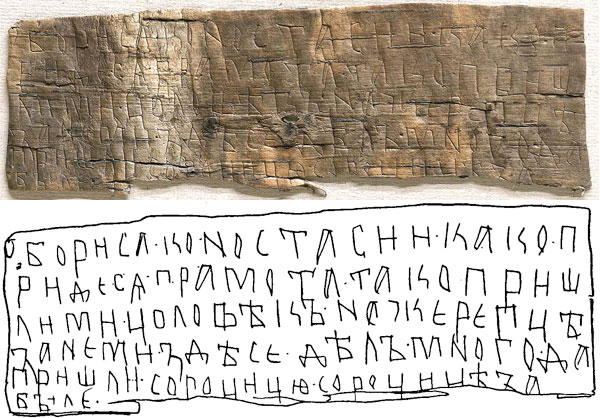
\includegraphics[width=0.95\textwidth]{fig/beresta}
    \end{center}
\end{frame}

\begin{frame}
    \frametitle{Литера}
    \framesubtitle{Математика на службе качества отображения глифа (изменить масштаб)}
    
    \begin{center}
        \begin{tabular}{c|c}
            \hline\hline
            Растр 
                & Вектор \\ \hline\hline
                & \\
            
\includegraphics[height=10pt]{fig/aletter}
                & $\mathcal{A}$ \\
                & \\ \hline
        \end{tabular}
    \end{center}
\end{frame}

\begin{frame}
    \frametitle{Код Морзе. Телеграф}
    
    \begin{center}
        \begin{tabular}{cl|cl|cl}
            \hline
            А/A   & \verb"• -    " & К/K & \verb"- • -  " & Ф/F   & \verb"• • - •  " \\
            Б/B   & \verb"- • • •" & Л/L & \verb"• - • •" & Х/H   & \verb"• • • •  " \\
            В/W   & \verb"• - -  " & М/M & \verb"- -    " & Ц/C   & \verb"- • - •  " \\
            Г/G   & \verb"- - •  " & Н/N & \verb"- •    " & Ч/    & \verb"- - - •  " \\
            Д/D   & \verb"- • •  " & О/O & \verb"- - -  " & Ш/    & \verb"- - - -  " \\
            Е,Ё/E & \verb"•      " & П/P & \verb"• - - •" & Щ/Q   & \verb"- - • -  " \\
            Ж/V   & \verb"• • • -" & Р/R & \verb"• - •  " & Ъ,Ь/X & \verb"- • • -  " \\
            З/Z   & \verb"- - • •" & С/S & \verb"• • •  " & Ы/Y   & \verb"- • - -  " \\
            И/I   & \verb"• •    " & Т/T & \verb"-      " & Ю/    & \verb"• • - -  " \\
            Й/J   & \verb"• - - -" & У/U & \verb"• • -  " & Я/    & \verb"• - • -  " \\
                  &                &     &                & Э/    & \verb"• • - • •" \\
            \hline
        \end{tabular}
    \end{center}
\end{frame}

SOS --- международный сигнал бедствия в радиотелеграфной связи с использованием азбуки Морзе. Это непрерывно повторяющаяся последовательность: три точки, три тире, три точки. Save Our Souls (Спасите наши души), Stop Other Signals (Остановите остальные сигналы), Спасите От Смерти, --- все эти пафосные расшифровки не отражают сути --- последовательность была выбрана исходя из удобства передачи. Современные радиоэлектронные средства передачи сигналов бедствия его уже не используют. 

Еще недавно радисты всего мира 48 раз в сутки, 2 раза каждый час (с 15-й по 18-ю минуту и с 45-й по 48-ю) обрывали на полуслове все сообщения, и настраивались на частоту 500 Гц в ожидании сигналов бедствия. Три минуты тишины в эфире.

Теперь этот сигнал стал полностью <<бытовым>> --- его легко передать например стуком по батарее, а на сигналы бедствия и аппаратуру существуют современные стандарты: .

Ходит легенда, что сигнал SOS впервые был передан погибающим Титаником. До этого использовался сигнал CQD --- Come Quick, Danger (Приходите Скорее, Опасность). Капитаны кораблей сигнал SOS якобы старались не использовать --- это был откровенный крик о помощи, прирзнание собственного бессилия. Титаник, несомненно передавал SOS, но однозначно сделал это не первым.

\begin{frame}
    \frametitle{Семафорная (флажковая) азбука}
    \framesubtitle{Служебные символы}
    
    \begin{center}
        \begin{tabular}{cl}
            
\includegraphics[height=45pt]{fig/semaphoreVyzov}   & Вызов \\
            
\includegraphics[height=45pt]{fig/semaphoreOtvet}   & Ответ (принял, понял) \\
            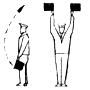
\includegraphics[height=45pt]{fig/semaphorePovtor}  & Повторение передачи (Ошибка)
        \end{tabular}
    \end{center}
\end{frame}

\begin{frame}
    \frametitle{Семафорная (флажковая) азбука}
    \framesubtitle{Служебные знаки при передаче букв}
    
    \begin{center}
        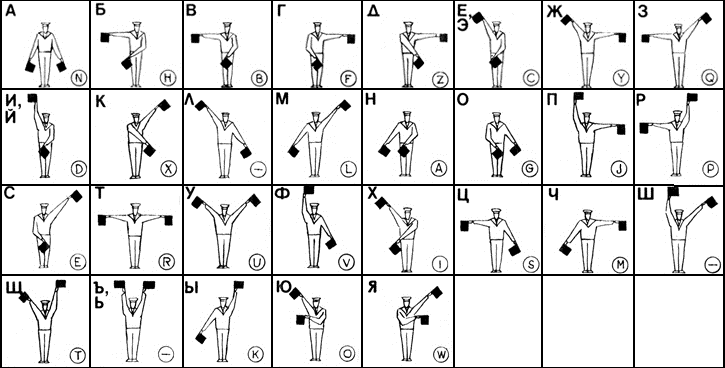
\includegraphics[width=0.9\textwidth]{fig/semaphore}
    \end{center}
\end{frame}

\begin{frame}
    \frametitle{Семафорная (флажковая) азбука}
    \framesubtitle{Морзянка}
    
    \begin{center}
        \begin{tabular}{cl|cl}
            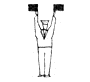
\includegraphics[height=45pt]{fig/semaphoreTochka}           & Точка &
                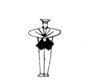
\includegraphics[height=45pt]{fig/semaphoreRazdelSymbol} & Разделитель тире и точек \\
            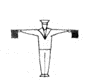
\includegraphics[height=45pt]{fig/semaphoreTire}             & Тире  &
                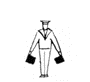
\includegraphics[height=45pt]{fig/semaphoreRazdelLetter} & Разделитель кодов букв, предложений \\
            &&
                
\includegraphics[height=45pt]{fig/semaphoreOshibka}      & Ошибка передачи, просьба повторить
        \end{tabular}
    \end{center}
\end{frame}

Применялась на флоте, для дальней передачи сообщений как на суше, так и на море. Может передаваться руками, бескозырками, с флажками --- выше дальность передачи. Как видно, семафорной азбукой можно передовать морзянку.

\begin{frame}
    \frametitle{Русская азбука глухих (дактильная азбука)}
    
    \begin{center}
        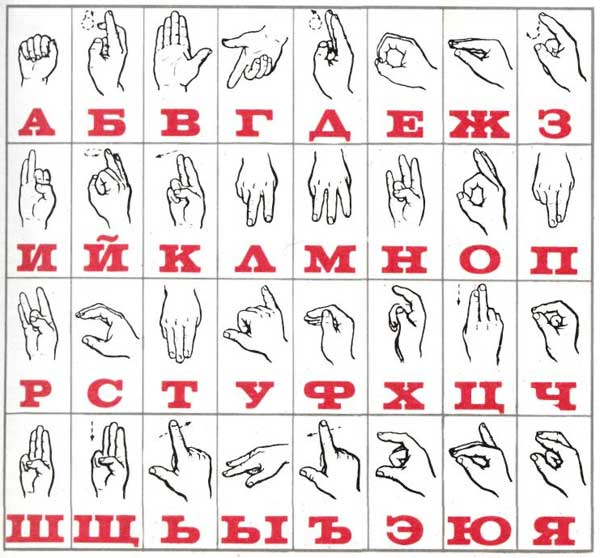
\includegraphics[width=.7\textwidth]{fig/dactile}
    \end{center}
\end{frame}

Азбука глухих может применяться не только глухими людьми. Это способ общения, когда нет возможности издавать звуки, но есть прямая видимость. Вас разделяет витрина магазина, вы в шумном помещении, вы аквалангист под водой.

Правая должна находиться на одном уровне с лицом, буквы артикулируются или проговариваются.

Отдельные жесты есть для обозначения месящев, дней недели, общеупотребимых понятий: учеба, вывеска, семья, дом школа. Для обозначения некоторых понятий комбинируются жесты, например, школа --- это жест учебы + вывеска.

\begin{frame}
    \frametitle{Азбука слепых (азбука Брайля)}
    \framesubtitle{Буквы}
    
    \begin{center}
        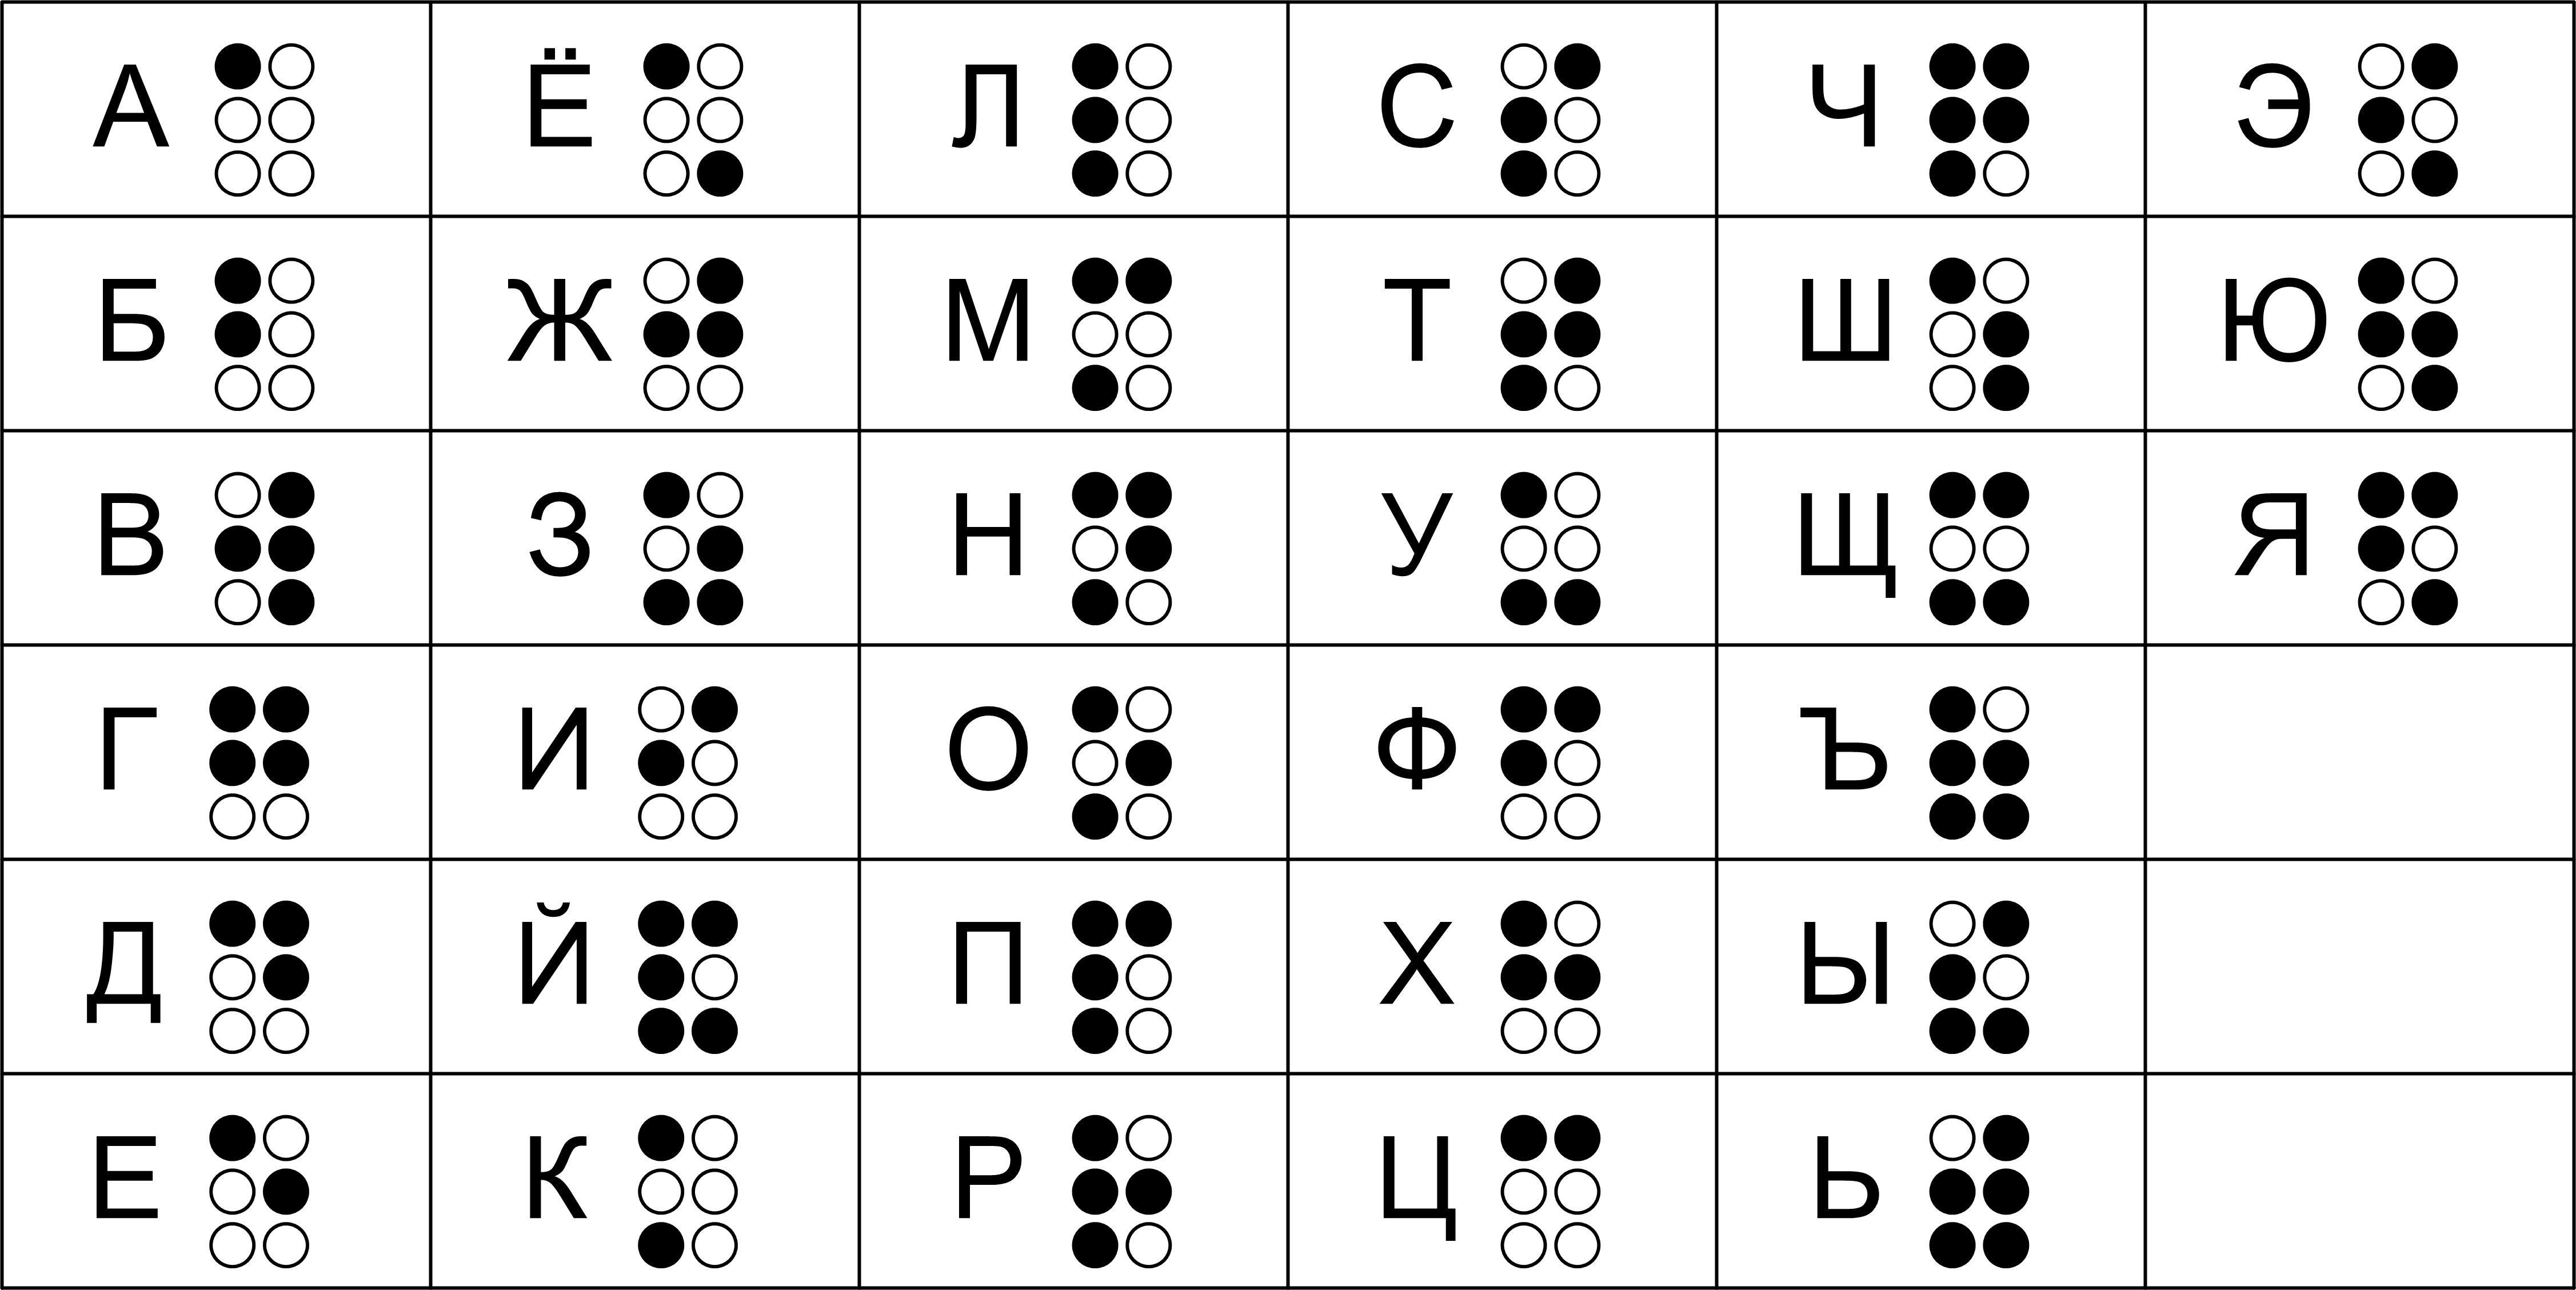
\includegraphics[width=.8\textwidth]{fig/braileLetters}
    \end{center}
\end{frame}

\begin{frame}
    \frametitle{Азбука слепых (азбука Брайля)}
    \framesubtitle{Цифры и математические знаки}
    
    \begin{center}
        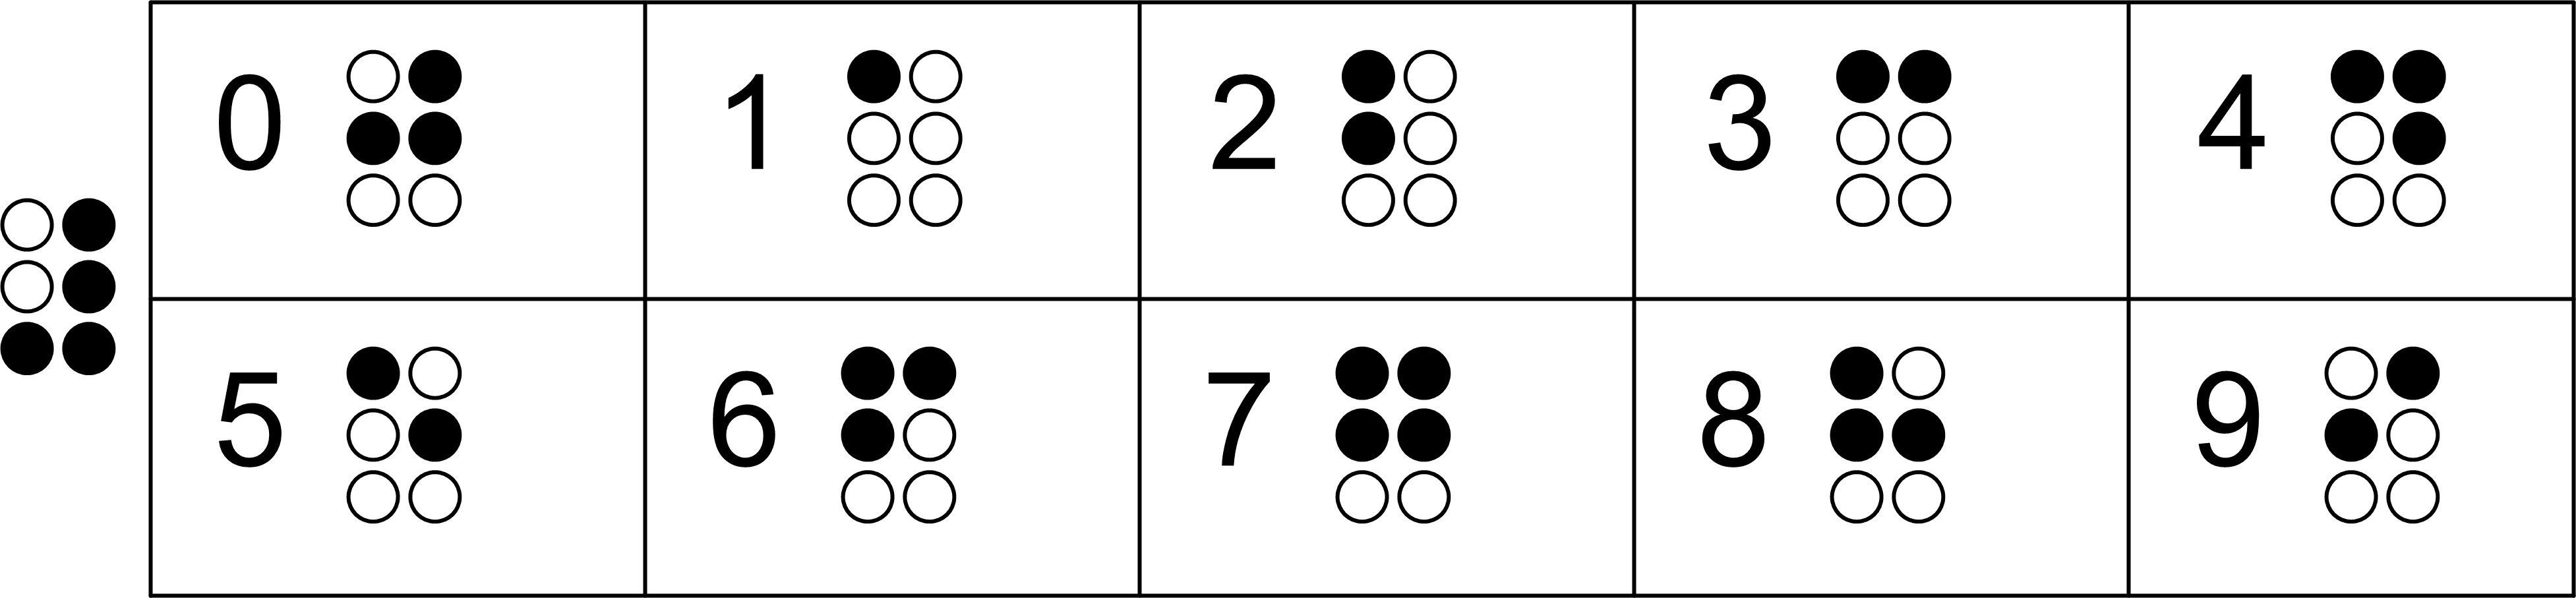
\includegraphics[width=.8\textwidth]{fig/braileDigits}
    \end{center}
    
    \begin{center}
        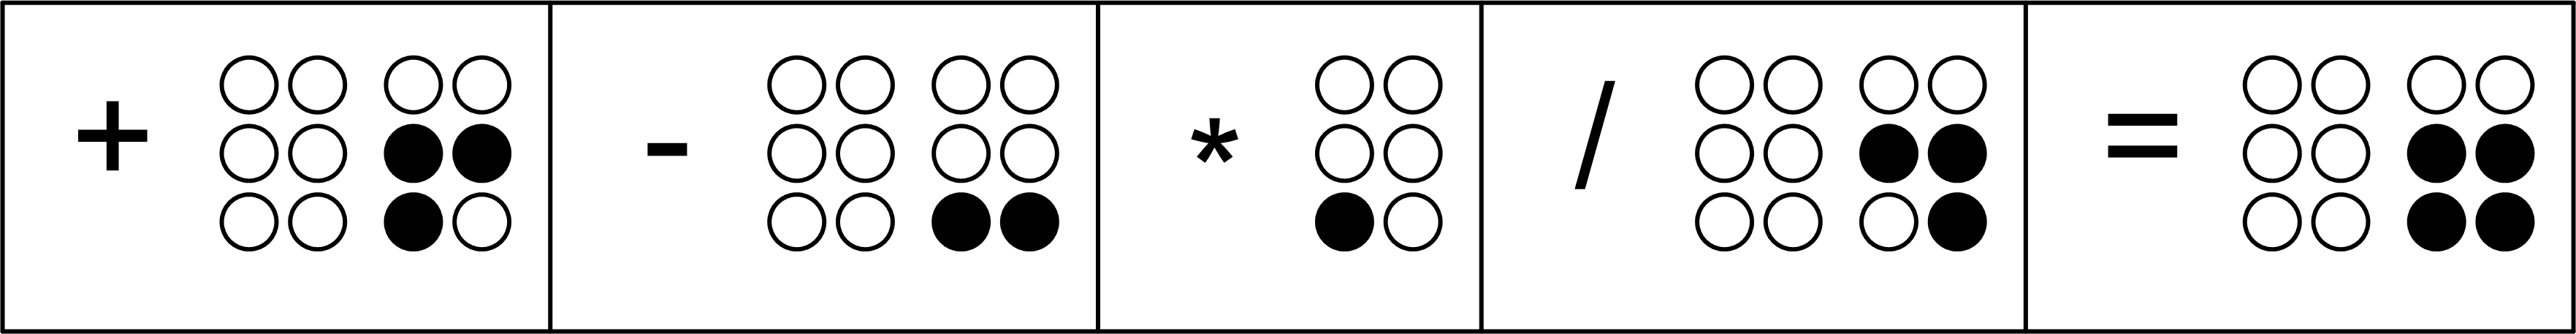
\includegraphics[width=.8\textwidth]{fig/braileMath}
    \end{center}
\end{frame}

\begin{frame}
    \frametitle{Азбука слепых (азбука Брайля)}
    \framesubtitle{Пунктуация}
    
    \begin{center}
        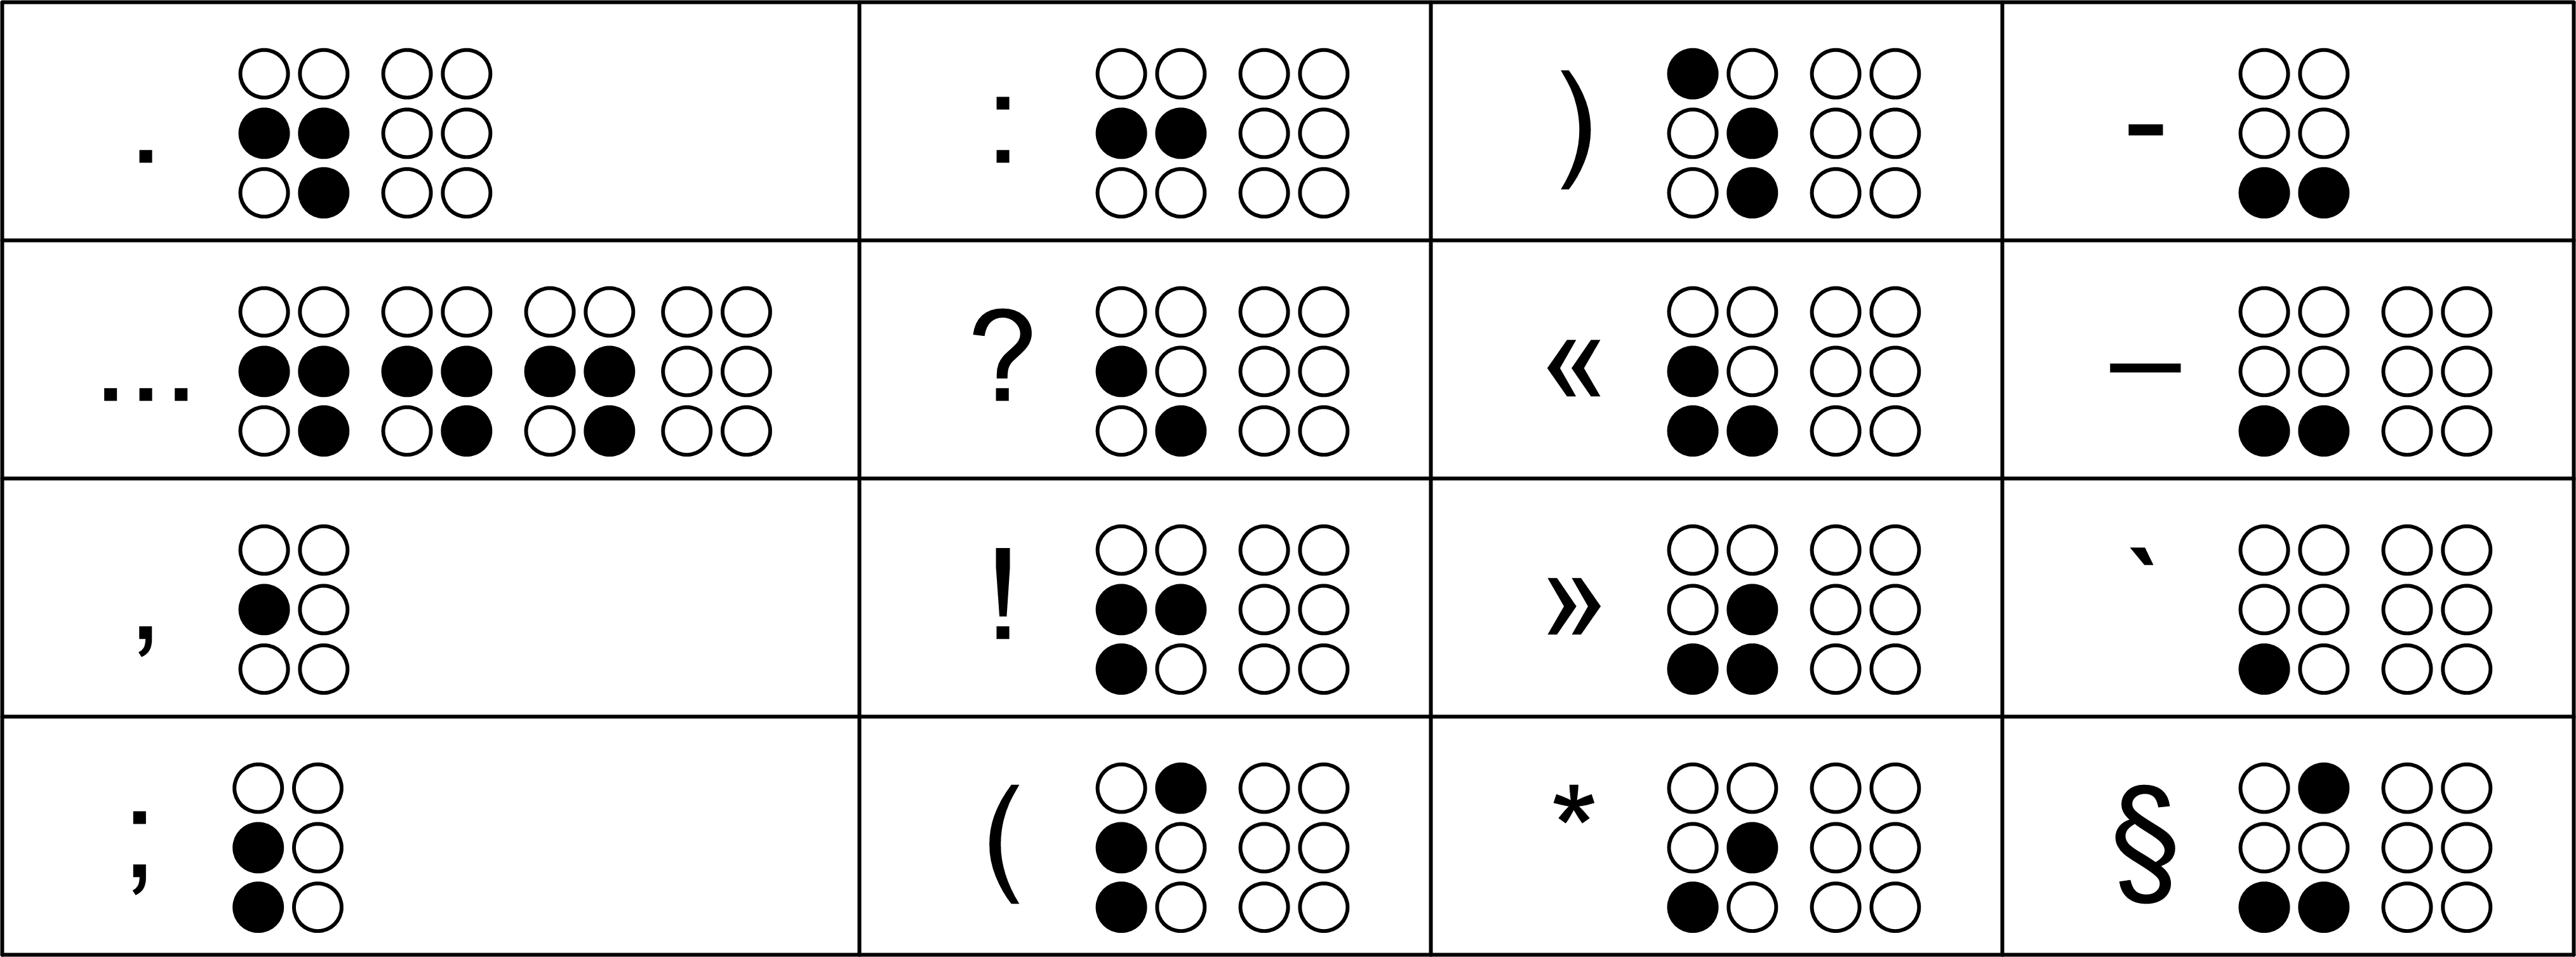
\includegraphics[width=.8\textwidth]{fig/brailePunctum}
    \end{center}
\end{frame}

\begin{frame}
    \frametitle{Азбука слепых (азбука Брайля)}
    \framesubtitle{Пример (\copyright http://pedlib.ru)}
    
    \begin{center}
        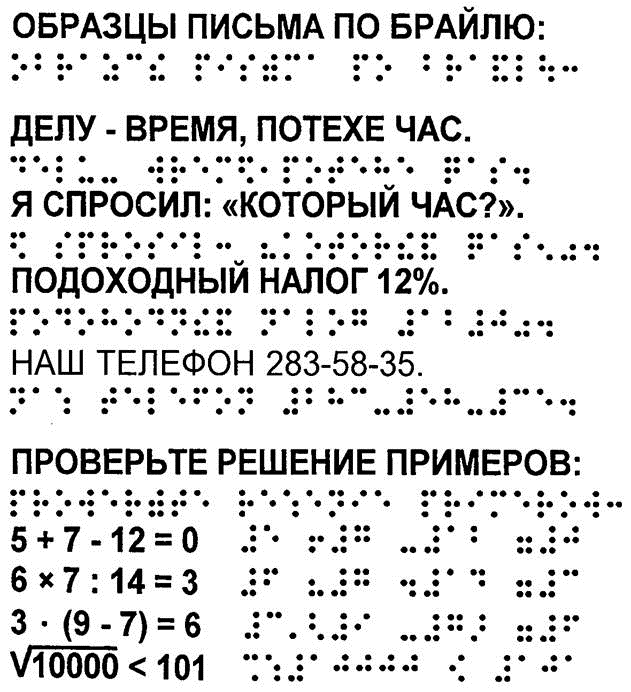
\includegraphics[height=.8\textheight]{fig/braileExample}
    \end{center}
\end{frame}

Шрифт брайля представлен в Unicode, правда восьмью точками. С 0x2800 по 0x28FF (c 10240 по 10495). Продемонстрировать в Word.

\begin{frame}
    \frametitle{Международный морской свод}
    \framesubtitle{Флаги}
    
    \begin{center}
        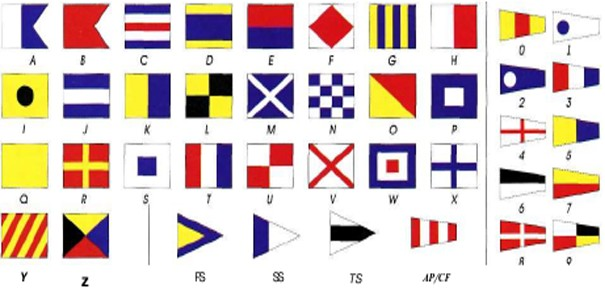
\includegraphics[width=.95\textwidth]{fig/signalFlags}
    \end{center}
\end{frame}

\begin{frame}
    \frametitle{Международный морской свод}
    \framesubtitle{Коды}
    
    \begin{center}
        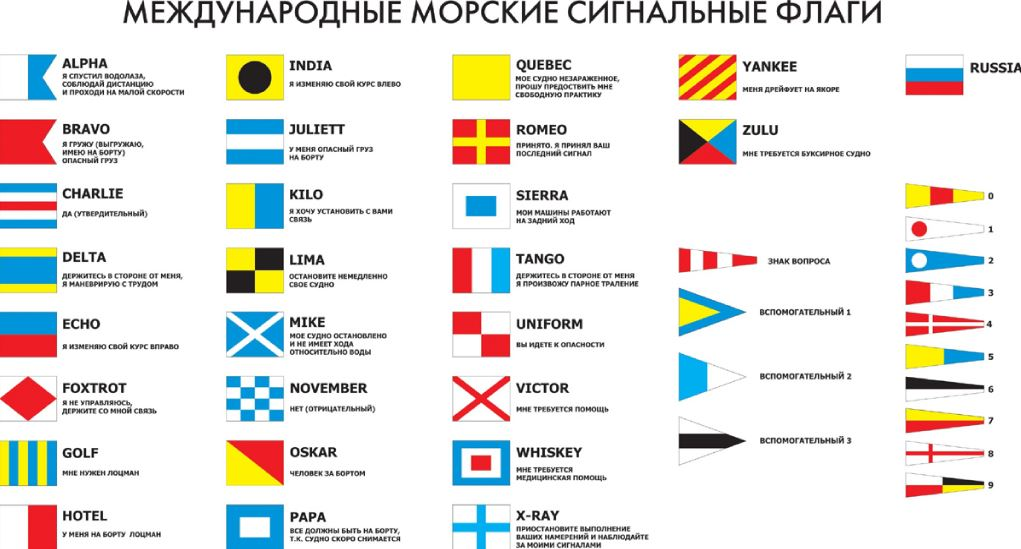
\includegraphics[width=.95\textwidth]{fig/signalFlagsCode}
    \end{center}
\end{frame}

\begin{frame}
    \frametitle{Международный морской свод}
    \framesubtitle{Примеры расшифровки кодов по МСС}
    
    \begin{itemize}
        \item A --- У меня спущен водолаз; держитесь в стороне от меня и следуйте малым ходом.
        \item О --- Человек за бортом.
        \item V --- Мне необходима помощь.
        \item W --- Мне необходима медицинская помощь.
        \item AR --- сигнал окончания, конец передачи или сигнала.
        \item CZ --- Вы должны стать бортом под ветер для приема шлюпки или плота.
        \item MAC --- Прошу вас договориться о госпитализации.
    \end{itemize}
\end{frame}

Флагу соответствует буква или цифра, есть также служебны флаги, например, использующиеся при нехватке обычных флагов.
В своде определены типовые ситуации на море. Свод издан на всех возможных языках морских держав. Например, ситуация: <<у меня спущен водолаз>>. Эти ситуации закодированы 1, 2 или 3 флаговыми комбинациями. Трехбуквенные комбинации относятся к медицинскому разделу и начинаются с буквы M.

Возможна передача слов на ланинице (открытым текстом), например названий судов.

Приняв сигнал, принимающая сторона поднимает вымпел (AP/CF) выше.

\begin{frame}
    \frametitle{Компьютерные таблицы кодов символов}
    \framesubtitle{American standard code for information interchange}
    
    \begin{center}
        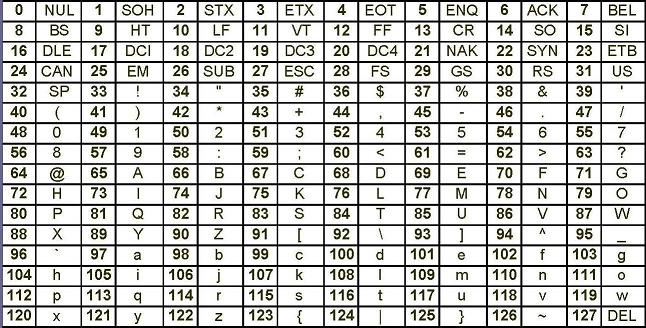
\includegraphics[width=.95\textwidth]{fig/ASCII}
    \end{center}
    Win: <<LAlt + Decimal-code>>
\end{frame}

\begin{frame}
    \frametitle{codepage866}
    
    \begin{center}
        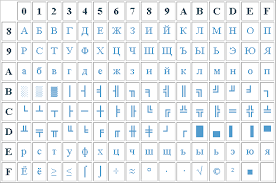
\includegraphics[width=.95\textwidth]{fig/cp866}
    \end{center}
\end{frame}

\begin{frame}
    \frametitle{codepage1251}
    
    \begin{center}
        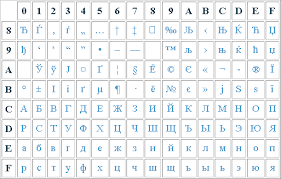
\includegraphics[width=.95\textwidth]{fig/cp1251}
    \end{center}
\end{frame}

\begin{frame}
    \frametitle{И пришел Unicode!}

    \url{http://unicode.org/}
    
    Единый стандарт на соотвествие кодов (номеров символов) глифам.
    
    \begin{block}{}
        Кодов гораздо больше, чем 256. Поэтому машинное представление номера символа в общем случае кодируется переменным количеством байт.
    \end{block}
    
    Способов представления номеров символов несколько. Наибольшее распространение получили:
    \begin{itemize}
        \item UTF-8 --- в ОС Linux, Unix, Windows.
        \item UTF-16 --- UEFI-Bios.
        \item и т.д.
    \end{itemize}
\end{frame}

\begin{frame}
    \frametitle{Unicode}
    \framesubtitle{Представление номеров символов UTF-8}
    
    \begin{center}
        \begin{tabular}{|l|c|c|}
        \hline\hline
        Диапазон номеров символов    
                          & Кол-во байт 
                              & Значащих бит                                            \\ \hline\hline
        00000000-0000007F & 1 & 7  \\ \hline 
            \multicolumn{3}{|l|}{Код: 0xxxxxxx (Совпадает с ASCII)                         } \\ \hline\hline
        00000080-000007FF & 2 & 11 \\ \hline 
            \multicolumn{3}{|l|}{Код: 110xxxxx 10xxxxxx                                    } \\ \hline\hline
        00000800-0000FFFF & 3 & 16 \\ \hline 
            \multicolumn{3}{|l|}{Код: 1110xxxx 10xxxxxx 10xxxxxx                           } \\ \hline\hline
        00010000-001FFFFF & 4 & 21 \\ \hline 
            \multicolumn{3}{|l|}{Код: 11110xxx 10xxxxxx 10xxxxxx 10xxxxxx                  } \\ \hline\hline
        00200000-03FFFFFF & 5 & 26 \\ \hline 
            \multicolumn{3}{|l|}{Код: 111110xx 10xxxxxx 10xxxxxx 10xxxxxx 10xxxxxx         } \\ \hline\hline
        04000000-7FFFFFFF & 6 & 31 \\ \hline 
            \multicolumn{3}{|l|}{Код: 1111110x 10xxxxxx 10xxxxxx 10xxxxxx 10xxxxxx 10xxxxxx} \\ \hline
        \end{tabular}
    \end{center}
\end{frame}

Посмотреть в Hex-редакторе коды символов. Рассказать о BOM (EF BB BF).

\begin{frame}
    \frametitle{Текстовый формат}
    \begin{itemize}
        \item Неделимой единицей текста является символ. 
        \item Все множество символов разделяют на отображаемые и управляющие. 
        \item Отображаемым символам соответствует определенное изображение (начертание, glyph – глиф).
        \item Служебные символы (ASCII) обрабатываются особо:
        \begin{itemize}
            \item{} <<CR>>(0xD,13) --- Carriage Return заставляет воображаемую печатную машинку сдвинуть печатающую головку в начало строки
    
            \item{} <<LF>>(0xA,10) --- Line Feed заставит выполнить переход на новую строку текста. 
    
            \item{} <<BS>>(8) --- Back Space осуществляет сдвиг печатающей головки на один шаг назад, что позволяло печатать диакрит\'{и}ческие знаки над буквами или печатать символ дважды, что давало эффект {\bf{жирного}} шрифта.    
        \end{itemize}
    \end{itemize}
\end{frame}

Далее мы рассмотрим кодирование текста с целью его представления в информационных системах. Неделимой единицей текста является символ. Все множество символов разделяют на отображаемые и управляющие. Отображаемым символам соответствует определенное изображение (начертание, glyph – глиф). Один и тот же символ (например, буква А) может быть начертан совершенно по-разному. Стилистика изображения символа задается шрифтом, который определяет отображение кода символа на глиф. Управляющие же символы предназначены для служебных целей. Например, у европейцев принято разбивать текст на строки, читаемые справа-налево, и располагать эти строки сверху-вниз. Встретившийся символ возврата каретки (обозначается <<CR>> – Carriage Return) заставляет воображаемую печатную машинку сдвинуть печатающую головку в начало строки, а символ перевода строки (обозначается <<LF>> – Line Feed) заставит выполнить переход на новую строку текста. К сожалению, исторически единства в вопросах перехода в начало новой строки нет. В Unix/Linux операционных системах для этого достаточно одного символа <<LF>>, в сетевых протоколах и в операционной системе Windows необходимы оба <<CR>><<LF>>, а в Mac OS используется <<CR>>. Поэтому иногда могут возникнуть проблемы с построчным отображением файла, созданным в другой операционной системе. Примером управляющего символа также может служить <<BS>> (Back Space), 

осуществлявший сдвиг печатающей головки на один шаг назад, что позволяло печатать диакритические знаки над буквами или печатать символ дважды, что давало эффект жирного шрифта.

\begin{frame}
    \frametitle{Скорость ввода текста}

    \begin{itemize}
        \item RS 232 --- от 50 до 115 000 baud (символ/с).
        \item USB 2.0 --- 480 Мib/s.
        \item USB 3.0 --- 4.8 Gib/s.
        \item Ethernet 1000Base-X --- 1000 Mb/s.
        \item PCI Express 3.0(x16 линий) --- 64 Gib/s.
    \end{itemize}

    \begin{block}{}
        "--* А я могу печатать со скоростью 600 знаков в минуту\footnote{Средняя скорость печати обученного слепому способу печати пользователя от 200 до 400 знаков в минуту. На незнакомых текстах зафиксирована чемпионская скорость 896 знаков, а на знакомых --- 1200 знаков!}!

        "--* OMG?!

        "--* Такая фигня получается!!!
    \end{block}
\end{frame}

Десять пальцев не глядя! Объяснить назначение пимпочек на крлавиатуре, схемы расстановки пальцев! Программы и ресурсы для тренировки десятипальцевого набора текста. Объем курсовой работы

\begin{frame}
    \frametitle{<<Слепой>> десятипальцевый способ набора}
    
    \begin{center}
        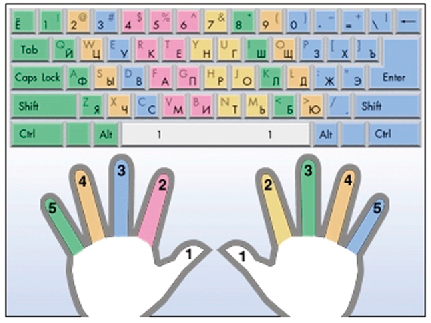
\includegraphics[width=.8\textwidth]{fig/tenfingers}
    \end{center}
\end{frame}

\begin{frame}
    \frametitle{Культовые текстовые редакторы}

    \begin{itemize}
        \item Sublime Text (Atom);
        \item Notepad++;
        \item Emacs;
        \item Vim;
        \item IDE (рефакторинг?);
        \item и т.д. На вкус на цвет\ldots
    \end{itemize}
\end{frame}

\begin{frame}
    \frametitle{Где используется текстовый формат (текст)}

    \begin{itemize}
        \item Исходные тексты программ.
        \item Языки разметки (Markup Languages) *ML.
        \begin{itemize}
            \item XML (SVG, MathMl, и т.д.).
            \item HTML.
            \item LaTeX.
        \end{itemize}
        \item Сетевые протоколы (HTTP, FTP, и т.д.).
        \item Донесение смысла до других (цель: образование \emph{общества} из популяции Homo Sapiens).
    \end{itemize}
\end{frame}

\begin{frame}
    \frametitle{Донесение смысла}

    Каждого ученика, подмастерья, стоящего на пороге любой профессии, где работать надо со словом, хорошо бы встречать примерно так:
    
    "--* Помни, слово требует обращения осторожного. Слово может стать живой водой, но может и обернуться сухим палым листом, пустой гремучей жестянкой, а то и ужалить гадюкой. И слово может стать чудом. А творить чудеса --- счастье. Но ни впопыхах, ни холодными руками чуда не сотворишь и Синюю птицу не ухватишь. Желаем тебе счастья!
    
    Скажут: для чудотворства ко всему нужен талант. Ещё бы!
    
    Чем больше талантов, тем лучше. Но надо ли доказывать, что и не обладая редкостным, выдающимся даром можно хорошо, добросовестно, с полной отдачей делать свое дело? А для этого нужно прежде всего, превыше всего --- знать, любить, беречь и никому не давать в обиду родной наш язык, чудесное русское слово.
    
    \begin{flushright}
        \copyright Нора Галь. <<Слово живое и мертвое>>
    \end{flushright}
\end{frame}

\begin{frame}
    \frametitle{Донесение смысла: информационный стиль}

    Десять правил сильного текста.
    \begin{enumerate}
        \item Сила --- в правде.
        \item Смысл важнее слов.
        \item Чем проще, тем лучше.
        \item Пишите как для себя.
        \item Читайте вслух.
        \item Приводите примеры.
        \item От простого к сложному.
        \item Пользу --- вперед.
        \item Поставьте заголовок.
        \item Уважение и забота.
    \end{enumerate}
    
    \begin{flushright}
        \copyright Максим~Ильяхов, Людмила~Сарычева: <<Пиши, сокращай>>.
    \end{flushright}
\end{frame}

- Донесение смысла
 -- Правила информационного стиля
  --- Канцелярит (Нора Галь)
 -- Составление резюме и сопроводительного письма.


\appendix

\begin{frame}
    \frametitle{Что почитать?}

    \begin{itemize}
        \item История развития систем передачи информации --- \cite{bib:souchek:noGolos}.
        \item О кодировании --- \cite{bib:petzold:code}.
        \item О том, как писать по-русски просто и сильно --- \cite{bib:gal:WordLiveAndDeath,bib:iliahov:writeShorter}.
    \end{itemize}
\end{frame}

\begin{frame}[allowframebreaks]{Библиография}
    \bibliographystyle{gost780u}
    \bibliography{./../../../bibliobase}
\end{frame}

\end{document}